\documentclass[a4paper]{article}
\usepackage[utf8]{inputenc}
\usepackage{enumitem}
\usepackage{url}
\usepackage{hyperref}
\hypersetup{
    colorlinks=true,
    linkcolor=blue,
    filecolor=magenta,      
    urlcolor=cyan,
}
\usepackage{caption}
\usepackage{color}

\definecolor{lightgray}{rgb}{.9,.9,.9}
\definecolor{darkgray}{rgb}{.4,.4,.4}
\definecolor{purple}{rgb}{0.65, 0.12, 0.82}

\usepackage{listings}
\lstset{basicstyle=\ttfamily,
  showstringspaces=false,
  commentstyle=\color{red},
  keywordstyle=\color{blue},
  captionpos=b,
  breaklines=true,
  backgroundcolor=\color{lightgray},
  columns=fullflexible,
}
\lstdefinelanguage{javascript}{
  keywords={typeof, new, true, false, catch, function, return, null, catch, switch, var, if, in, while, do, else, case, break},
  keywordstyle=\color{blue}\bfseries,
  ndkeywords={class, export, boolean, throw, implements, import, this},
  ndkeywordstyle=\color{darkgray}\bfseries,
  identifierstyle=\color{black},
  sensitive=false,
  comment=[l]{//},
  morecomment=[s]{/*}{*/},
  commentstyle=\color{purple}\ttfamily,
  stringstyle=\color{red}\ttfamily,
  morestring=[b]',
  morestring=[b]"
}


% *** GRAPHICS RELATED PACKAGES ***
%\usepackage[pdftex]{graphicx}
\usepackage{graphicx}
%\usepackage[dvips]{graphicx}
% to place figures on a fixed position
\usepackage{float}

\usepackage[margin=1in]{geometry}

\title{Blockchains for Industrial IoT - a Tutorial}

\author{Pal Varga and Ferenc Janky \\ Budapest University of Technology and Economics}


\date{v0.9 \\ 2019}

\begin{document}

\maketitle

\begin{abstract}
Utilizing Blockchains within the Internet of Things (IoT) concept is quite a recent idea. There are already a number of use cases and supporting frameworks available, which shows its potential benefits for many domains.

There are interesting, business-driven target areas within the Industrial IoT domain, including sectors such as supply chain (including manufacturing, transportation and logistics), maintenance, energy trading, grids, and even healthcare. When compared to consumer IoT, these systems have special requirements: certain level of real-time, security, engineering complexity, multi-stakeholder visibility, fast transaction and asset traceability. While the Distributed Ledger Technology (DLT) already addresses some areas of these (such as multi-stakeholder visibility or asset traceability), Blockchain Technology (BCT) provides additional value for security, building trust, and reducing cost while accelerating transactions of service agreements.
This tutorial aims to reveal the opportunities and challenges as well as presenting real-life examples together with network management aspects. First it provides an overview and definitions the BCT universe – from Assets and Blocks through Consensus Mechanisms and Distributed Ledgers to Wallets. Next, it describes some special requirements of the Industrial IoT domain together with ideas of utilizing BCT to cover these needs. While discussing benefits, the tutorial reveals some drawbacks as well. These help us answering the questions: when is it beneficial to use BCT, when is it questionable, and when is it avoidable?

Furthermore, the tutorial provides insights on various use-cases of employing BCT and smart service contracts in healthcare, electricity trading, production, asset tracking or proactive maintenance. Aside from being interesting simply because they are becoming core technologies of near-future systems, IIoT and Blockchains have a network management viewpoint as well. The IIoT end-devices need on-boarding, their data needs to be secured, authenticity needs to be checked, and trust needs to be built – all of which tasks BCT can be utilized effectively. Moreover, as part of configuration management, reliable and secure firmware distribution and upgrade can be supported inherently.

The hands-on part of this tutorial includes a multi-player bidding scenario.  In here, the users (consumers) can deploy smart service contracts on in an Ethereum-based blockchain, stating their need of given amount of energy at a maximum price. The energy-provider type of players in this scenario can bid on winning the contract. The various transactions related to the bidding, energy consumption and withdrawal of gains can be followed by the players either by using the GUI provided, or by issuing commands for reading transaction parameters and service contract values stored at the blockchain.

\end{abstract}

\newpage

\tableofcontents

%\newpage

\section{Introduction}

This tutorial provides a generic overview of Blockchain Technology and its feasibility for the  Industrial Internet of Things (IIoT) domain. The tutorial itself consist of three parts: (i) an oral lecture with its separate presentation material, (ii) the current syllabus providing support background material for (iii) the demo on using smart service contracts in a multi-player bidding scenario.

In order to get a proper grip on the tutorial exercises, some of the main concepts of the Blockchain Technology, the Distributed Ledgers, and the Smart Service Contract are described here.
Beside this, some of the application areas of these concepts for Industrial Internet of Things (IIoT) are discussed in brief.

The presentation material is also available for this tutorial, at ...

The demo application for the multi-player bidding scenario is available at ...


\section{Motivation: using Blockchains for Industrial IoT}

\subsection{Generic considerations}

Special features and requirements of IIoT

Criteria on Real-time, Security, Trust, Engineering efficiency, etc.

\subsection{A short overview of IoT security: issues and solutions}

\subsection{Special features of Blockchains to be utilized by IIoT}

\subsubsection{Interoperability across IoT devices, IoT systems and industrial sectors}
\subsubsection{Traceability and Reliability of IoT data}
\subsubsection{Improved Security of IoT systems}
\subsubsection{Autonomic interactions of IoT systems}

security, anonymity and data privacy, trust, accelerated transactions, micropayments, ledger as a distributed and trusted database, cost reductions by removing middlemen, etc.

Which kinds of IoT security issues can be covered by BCT, and how?

\subsubsection{Precautions for Blockchain usage}

Vulnerabilities, Risks, Mitigation. Legal issues

\subsection{When is it beneficial to use BCT for IIoT?}

Figure~\ref{fig:BC_Do_You_Need} depicts one of the rule-of-the-thumb decision diagrams on the topic.
%\begin{lstlisting}[language=python,frame=single,breaklines]
%packet = event.parsed  
%\end{lstlisting}
\begin{figure}[H]
    \centering
    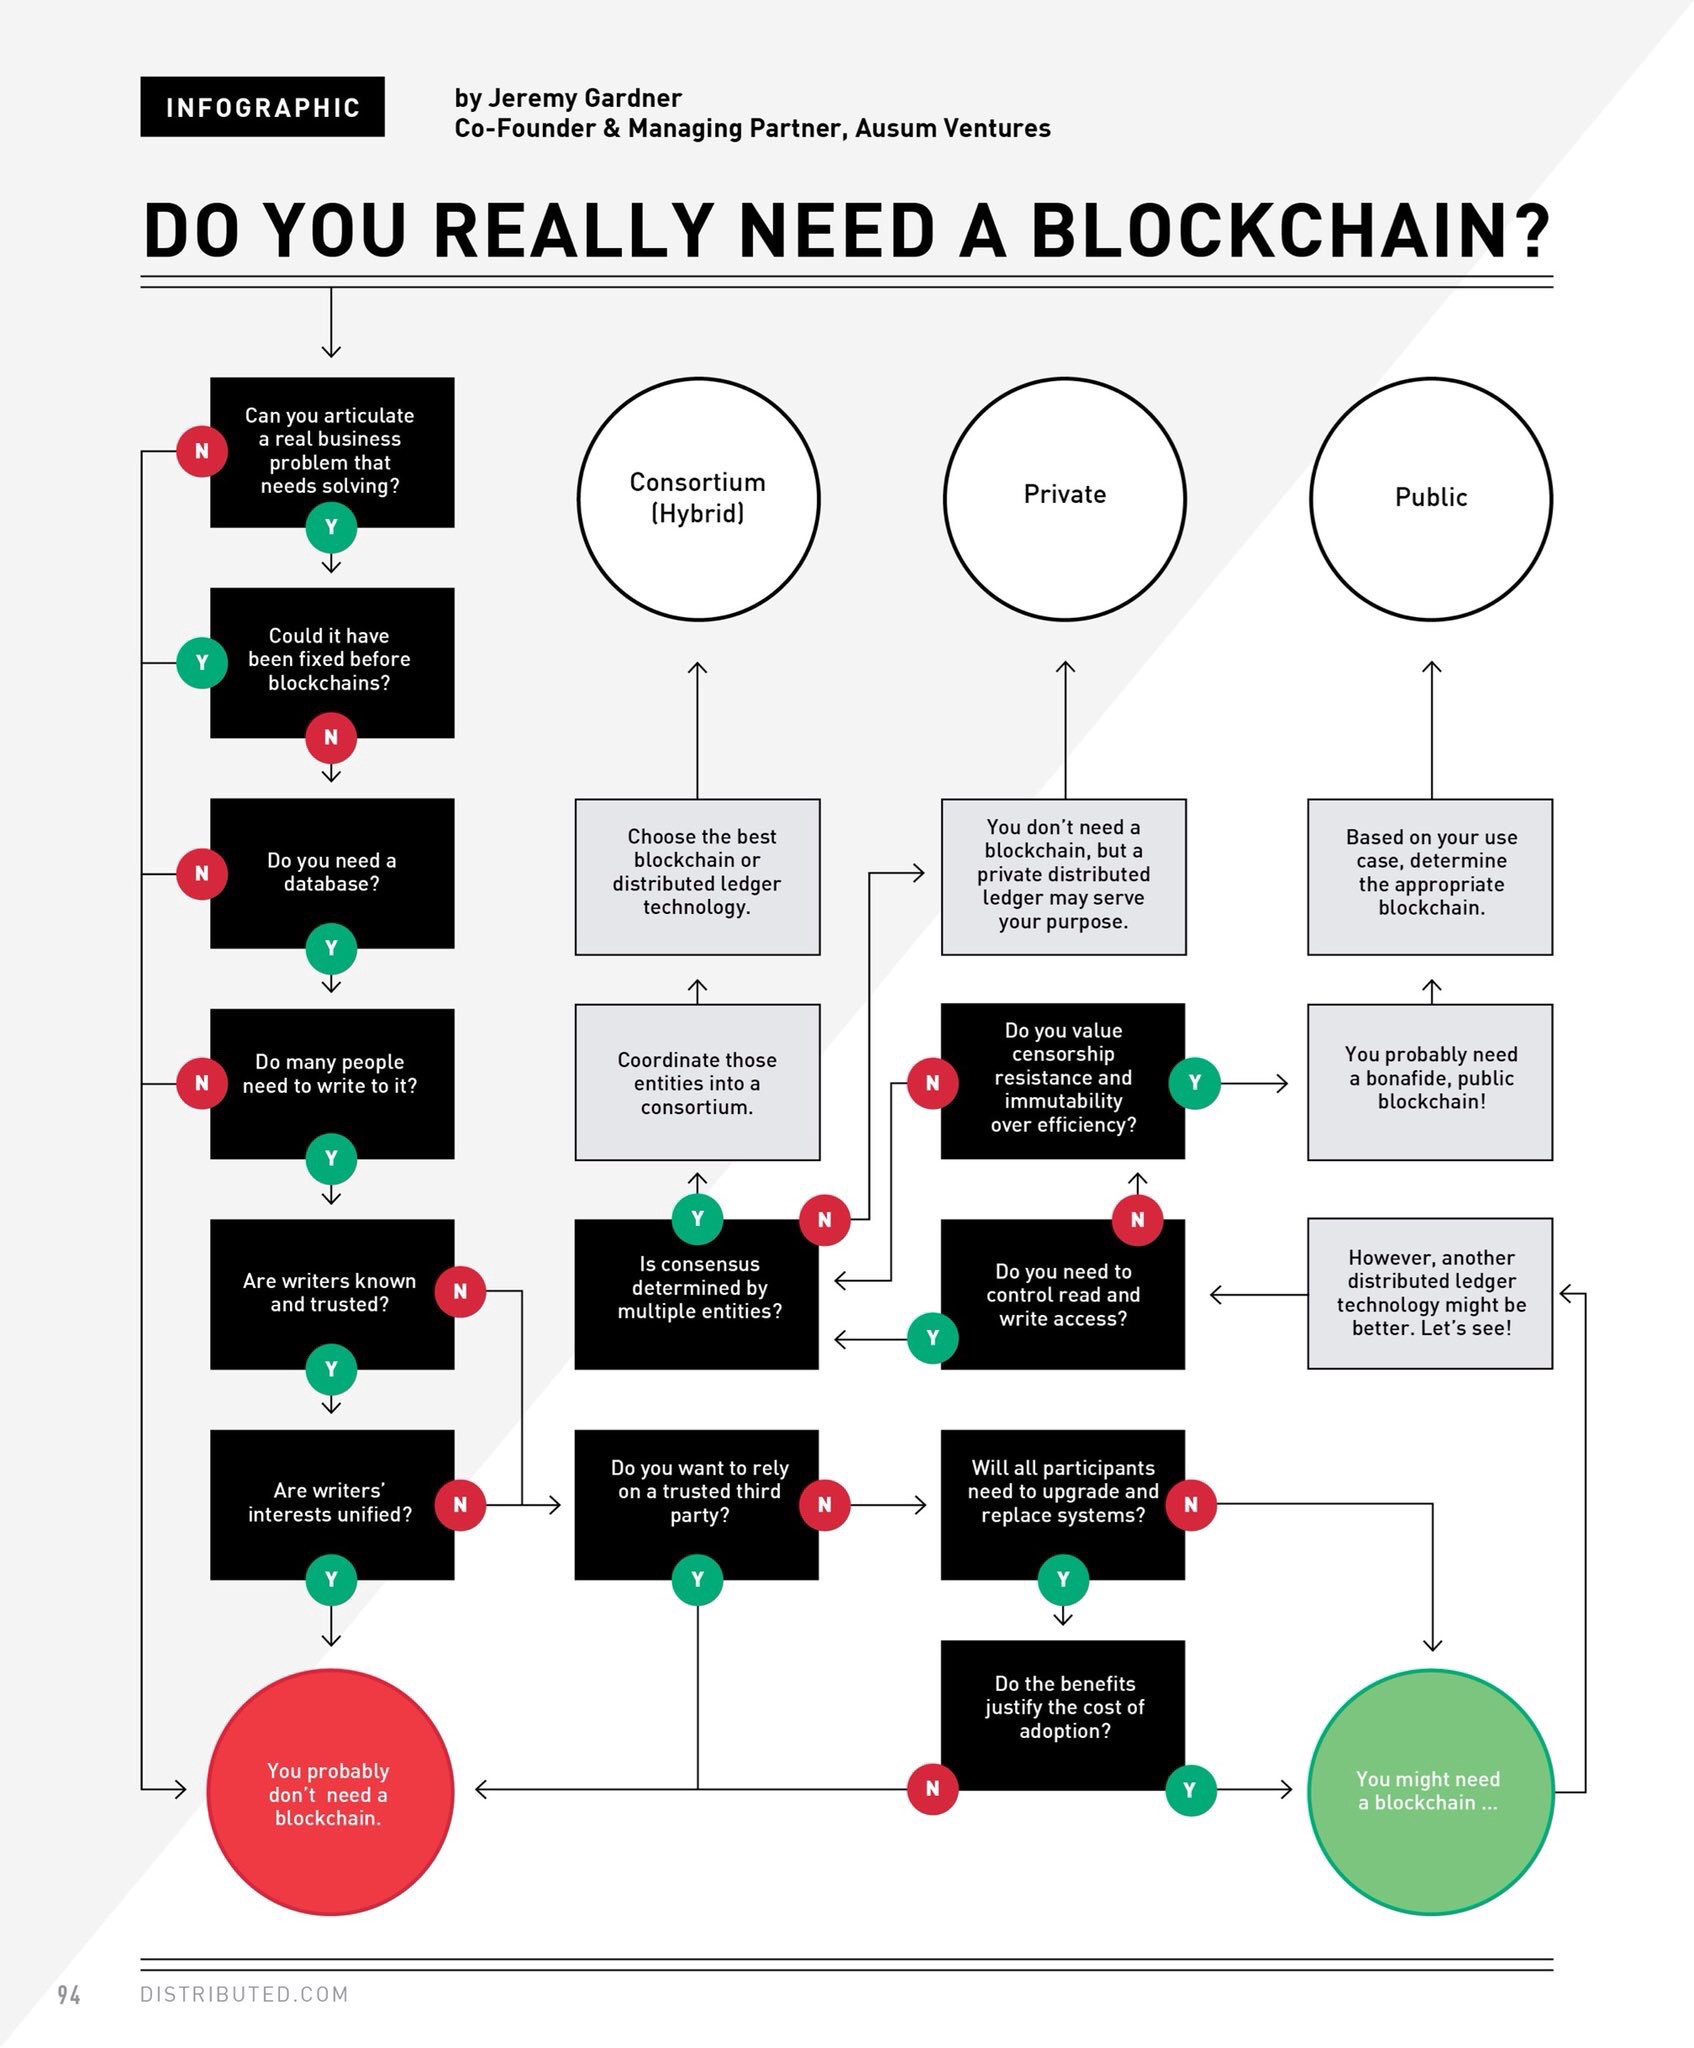
\includegraphics[width=0.95\textwidth]{figures/DoYouNeedBC.jpg}
    \caption{Do You Need to use Blockchains? (by Jeremy Gardner, 2018)}
    \label{fig:BC_Do_You_Need}
\end{figure}


\section{Blockchain-related concepts}

This subsection aims to provide some basic references related to Blockchains. This document merely provides some initial definition together with citing references that further elaborate either the whole topic or the given term. Providing a comprehensive overview of the terms is outside of the scope of this document.

Nevertheless, readers are encouraged to check out the cited further resources and targeted tutorials on these concepts. The cited references are deliberately chosen from various sources to show the wide range of tutorial materials available for readers at various levels of interest. 

\subsubsection{Blockchain}
As $techterms.com$ \cite{techterms} defines (with slight additions):
\begin{quote}
    "A blockchain is a digital record of transactions. The name comes from its structure, in which individual records, called blocks, are linked together in single list, called a chain. Blockchains are used for recording transactions made with cryptocurrencies, such as Bitcoin, and have many other applications -- including smart service contracts for IoT.
    
    Each transaction added to a blockchain is validated by multiple computers on the Internet or on intranets of private operators. These systems, which are configured to monitor specific types of blockchain transactions, form a peer-to-peer network. They work together to ensure each transaction is valid before it is added to the blockchain. This decentralized network of computers ensures a single system cannot add invalid blocks to the chain.
    
    When a new block is added to a blockchain, it is linked to the previous block using a cryptographic hash generated from the contents of the previous block. This ensures the chain is never broken and that each block is permanently recorded. It is also intentionally difficult to alter past transactions in blockchain since all the subsequent blocks must be altered first."
\end{quote}

\subsection{A sample workflow of Blockchain-related processes}

Figure~\ref{fig:BC_Workflow} depicts a sample workflow.
%\begin{lstlisting}[language=python,frame=single,breaklines]
%packet = event.parsed  
%\end{lstlisting}
\begin{figure}[H]
    \centering
    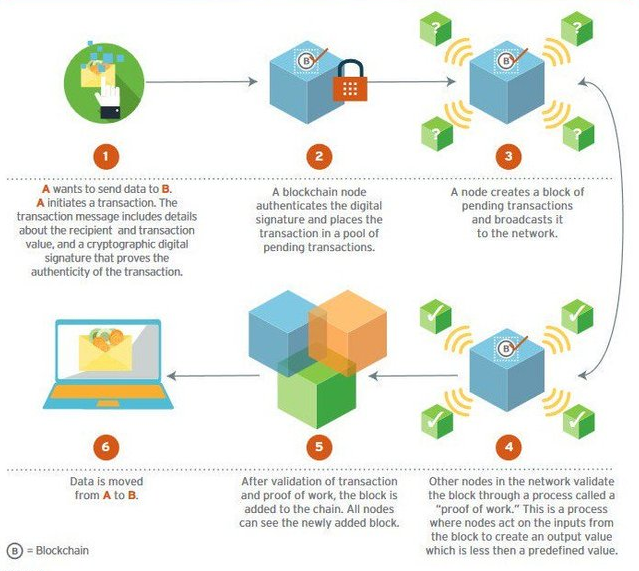
\includegraphics[width=0.95\textwidth]{figures/sample_BC_flow.png}
    \caption{A typical workflow of a Blockchain-related process (https://steemit.com/blockchain/)}
    \label{fig:BC_Workflow}
\end{figure}

\subsubsection{Distributed Ledger Technology}
The distributed ledger database is spread across several nodes (devices) on a peer-to-peer network, where each replicates and saves an identical copy of the ledger and updates itself independently. The primary advantage is the lack of central authority. When a ledger update happens, each node constructs the new transaction, and then the nodes vote by consensus algorithm on which copy is correct. Once a consensus has been determined, all the other nodes update themselves with the new, correct copy of the ledger \cite{DLT}.


\subsubsection{Cryptographic Hash Function}
The reason to apply "hashing" on data (or the "message") put on the blockchin is making it secret so only those with proper access rights can read it, and second, making it immutable: if the message is modified, the hash value will change. After such change, it is impossible to reconstruct the original message.

A cryptographic hash function (CHF) is a hash function that is suitable for use in cryptography. It is a mathematical algorithm that maps data of arbitrary size to a bit string of a fixed size (the "hash value", "hash", or "message digest") and is a one-way function, that is, a function which is practically infeasible to invert \cite{CHF}.

\subsubsection{Mining}

Once a message is hashed, it gets broadcasted among all the mining nodes so it would become part of a block on the chain. Mining is the process of adding transaction records to a ledger of past transactions --, i.e., the blockchain. The blockchain serves to confirm transactions to the rest of the network as having taken place. 

As the network nodes are widely distributed, every miner in the network is expected to receive multiple messages from multiple vendors at any given period of time. What the miner does is he combines these messages in a single block \cite{tutorialspoint}.

The primary purpose of mining is to set the history of transactions in a way that is computationally impractical to modify by any one entity. By downloading and verifying the blockchain, the nodes are able to reach consensus about the ordering of events. 

Mining is intentionally designed to be resource-intensive and difficult so that the number of blocks found each day by miners remains steady. Individual blocks must contain a proof (e.g. proof of stake, proof of stake, etc.) to be considered valid. This proof is verified by other blockchain nodes each time they receive a block \cite{bitcoin_wiki}.

\subsubsection{Consensus algorithms}
One of the outcomes of the mining procedure is to validate the transactions of a block. As part of this, miners are working to find a $nonce$ that shows that the block hash satisfies an earlier-defined, well-known target criterion.

The Proof of Work (PoW) is a popular consensus algorithm; and as such, it is aimed for resolving the problem of reliability in a network involving multiple unreliable nodes. The PoW is deliberately computationally intensive for miners. It is a piece of data which is difficult (costly, time-consuming) to produce but easy for others to verify and which satisfies certain requirements. Producing a proof of work can be a random process with low probability so that a lot of trial and error is required on average before a valid proof of work is generated \cite{tutorialspoint}, \cite{bitcoin_wiki}.

There are several other consensus algorithms exists \cite{consensus}, one of the well known ones beside PoW (used by e.g. Bitcoin) is Proof of Stake (used by e.g. Ethereum), where the creator of the next block is called "validator" (instead of miner) and is chosen via various combinations of random selection and wealth or age (i.e., the stake).  
%\subsubsection{Practical Byzantine Tault Tolerance}

\subsubsection{Merkle Tree}

In order to help compressing blockchain data for those nodes who are not interested in mining, but only exchanging goods, writing messages on the blockchain and checking whether a transaction is valid that is on the blockchain, the binary Merkle Hash Tree (see Figure~\ref{fig:merkle}) can be used.

\begin{figure}[H]
    \centering
    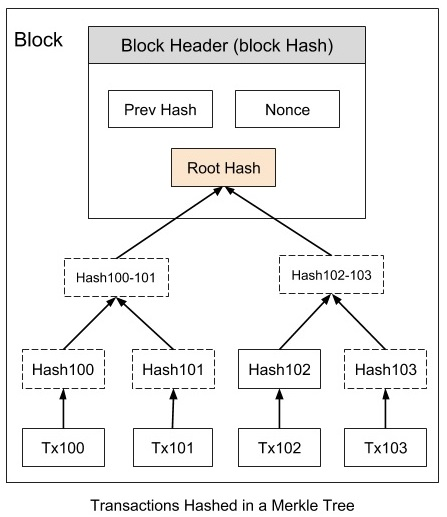
\includegraphics[width=0.5\textwidth]{figures/merkle_tree.jpg}
    \caption{Merkle Tree \cite{tutorialspoint}}
    \label{fig:merkle}
\end{figure}

When transactions hashed into a Merkle Tree, the client merely need to have the Previous hash, the Merkle Root, and the Nonce for Each Block header - as Figure~\ref{fig:merkle_verif} shows. 

\begin{figure}[H]
    \centering
    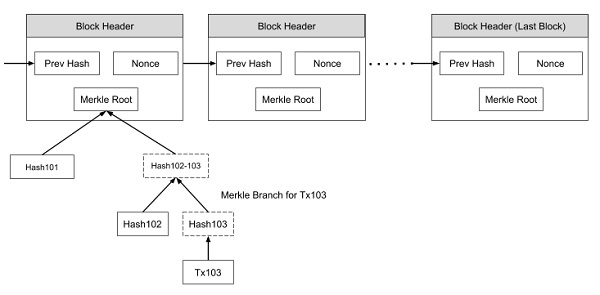
\includegraphics[width=0.9\textwidth]{figures/payment_verification.jpg}
    \caption{Transaction verification by using the Merkle Root \cite{tutorialspoint}}
    \label{fig:merkle_verif}
\end{figure}

In order to verify certain transactions made in the past, the Merkle Roots and corresponding hashes need to be used instead of all hashes for the given transactions on the block \cite{IOTA_Merkle}. 



\subsection{Smart Contracts}

\subsection{Issues related to the IIoT domain}


\section{Smart contracts using Ethereum}

Within the Ethereum framework Smart Contracts are implemented in the form of Decentralized Applications - DApp. These DApps are defined using a higher level programming language that is either :
\begin{itemize}
    \item Solidity, that is a statically typed programming language showing similarities to Javascript, C++ and other high level, object oriented languages \cite{solidity_manual}
    \item Vyper, which is a Python based language still under development \cite{vyper_doc}
\end{itemize}

Smart contracts defines the data and the protocol on how that data can be changed. Actually since one key feature is that blockchains are immutable change might not be the appropriate term for that but more like how the data should be transformed to get in to a next valid state. This is analogous to various well established immutable algorithms and data structures like: persistent list, m-trie, etc. \cite{persistent_data_structures} 

\subsection{Concepts}\label{sec:EthSmartContracConcepts}

The process of how a smart contract is synthesized onto "executable code" is somewhat similar to other well known 
Data and code is stored on the blockchain, code can be called using a well known ABI. etc. Add figure on how this adds up

\subsubsection{Simplified concept of Smart Contract operation}
\begin{figure}[H]
    \centering
    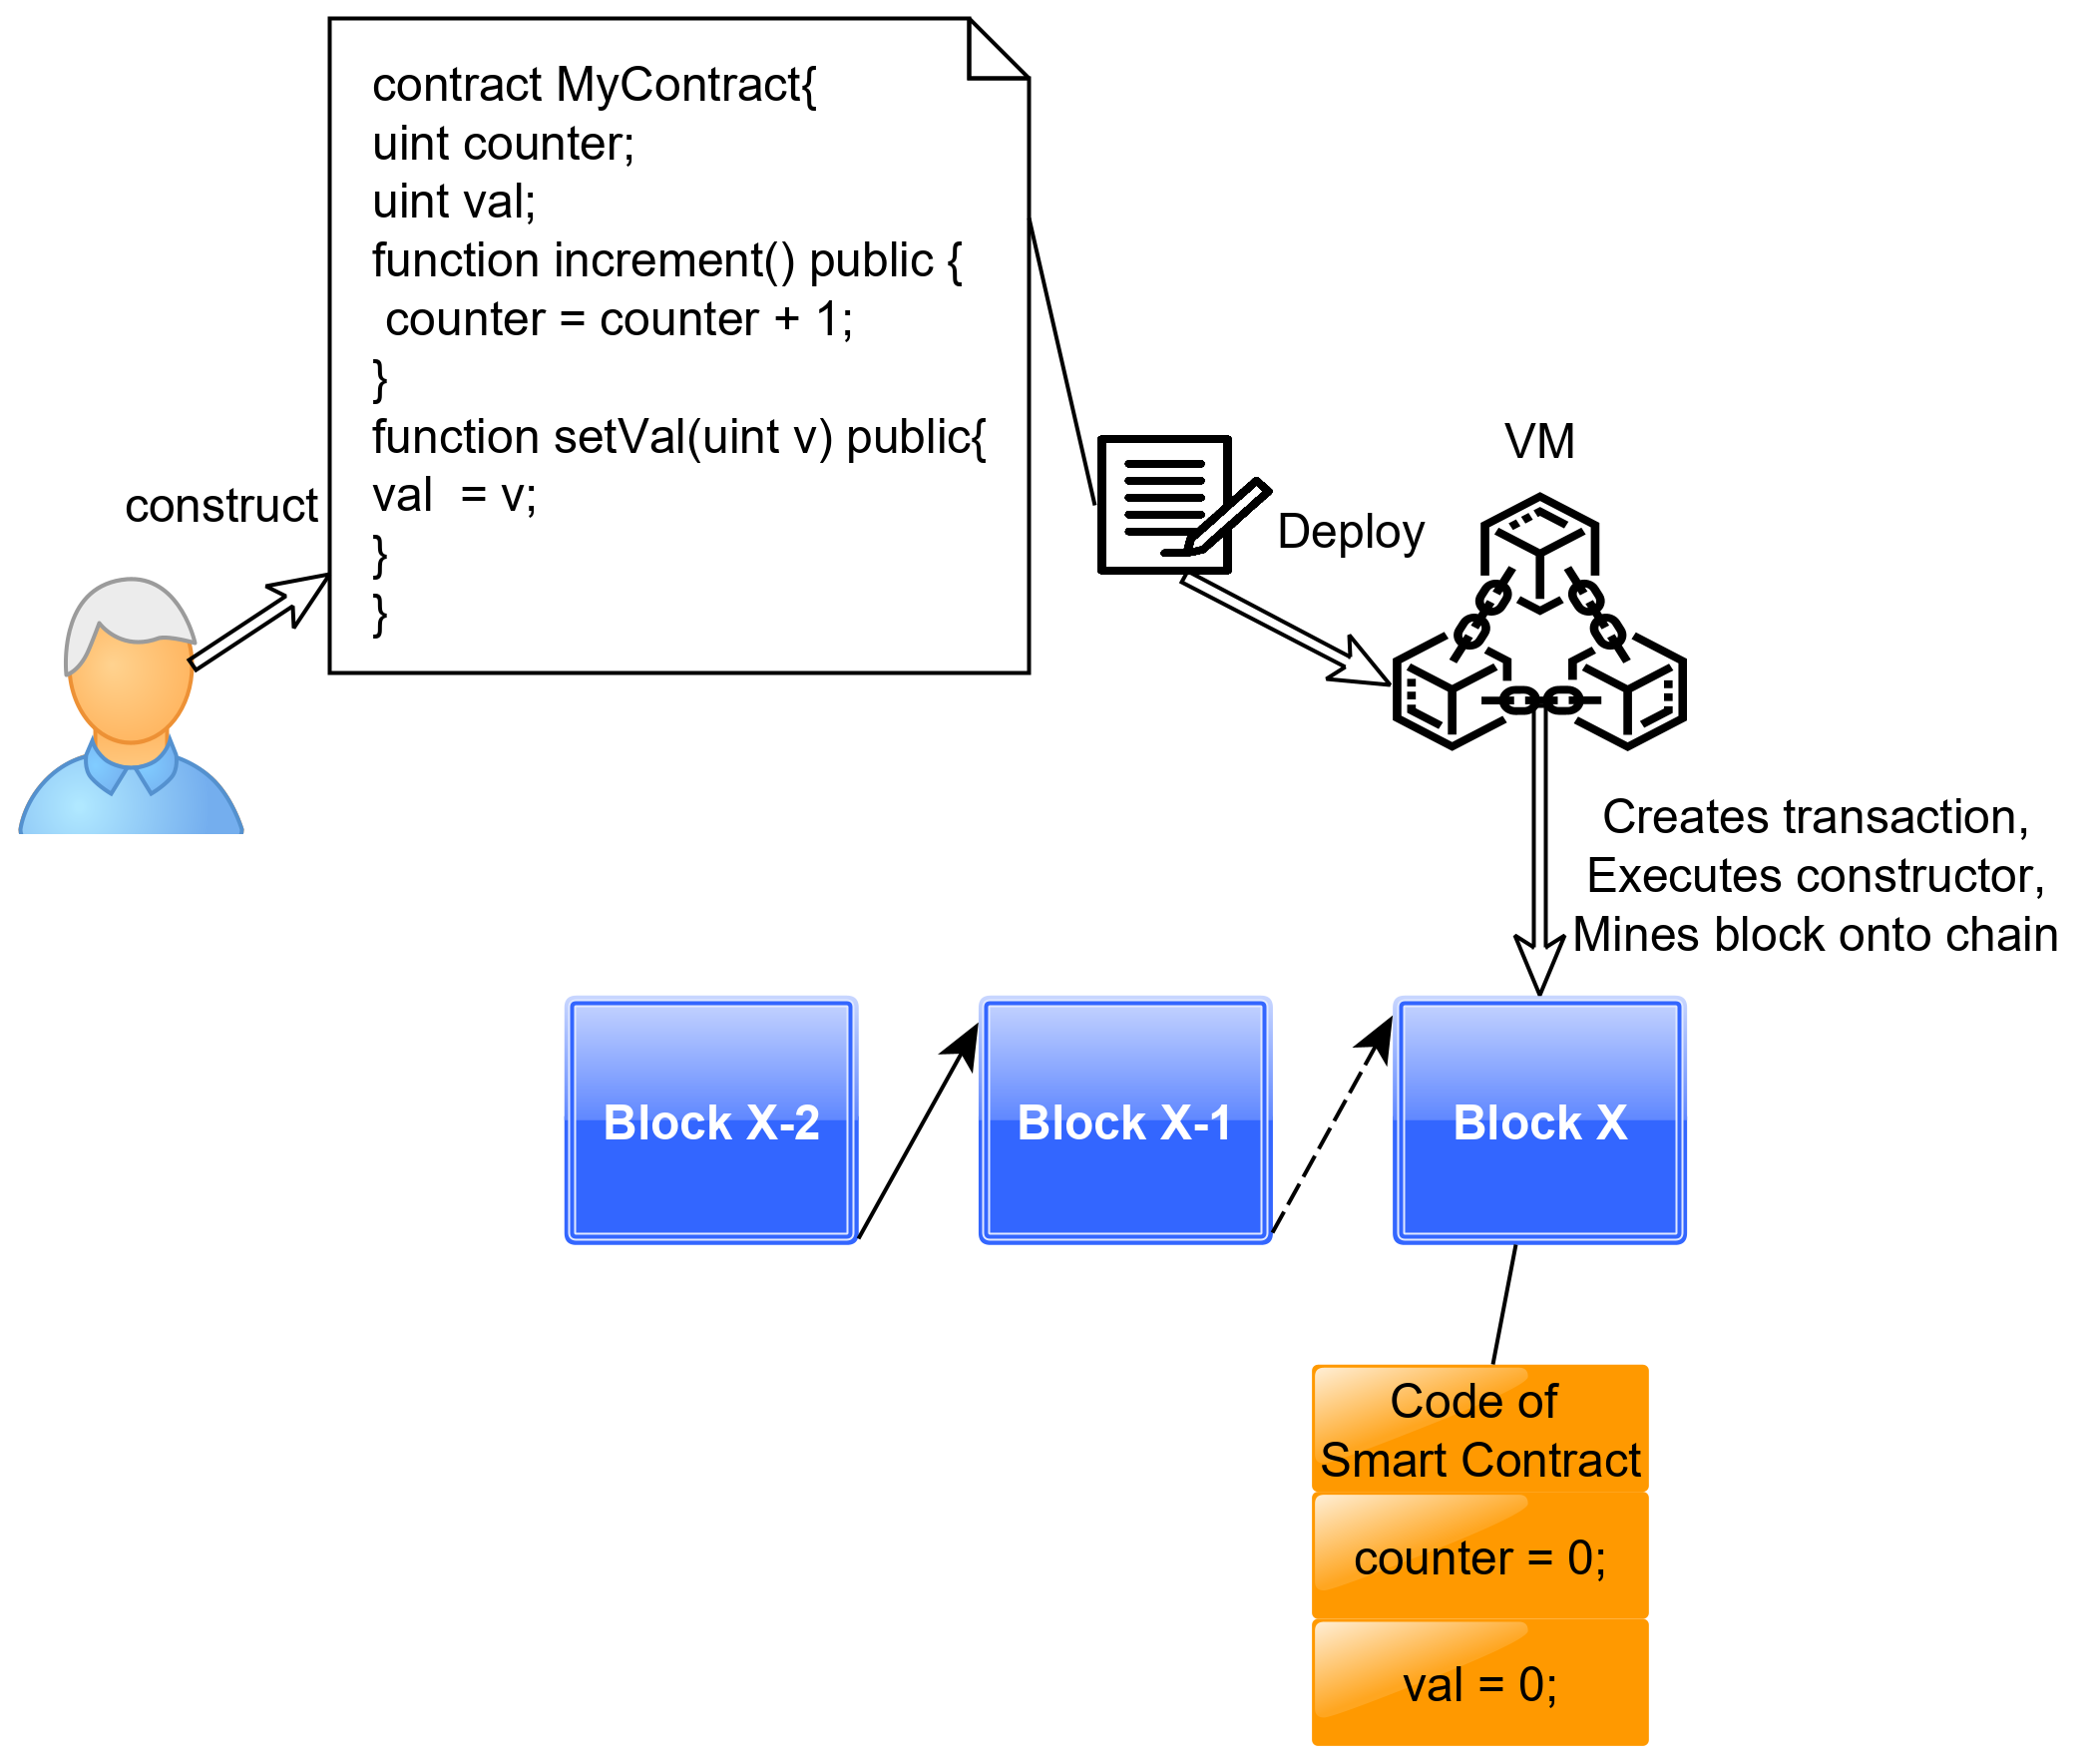
\includegraphics[width=0.9\textwidth]{figures/deploy_0.png}
    \caption{User constructs smart contract, VM deploys it onto the chain}
    \label{fig:deploy_0}
\end{figure}
\begin{figure}[H]
    \centering
    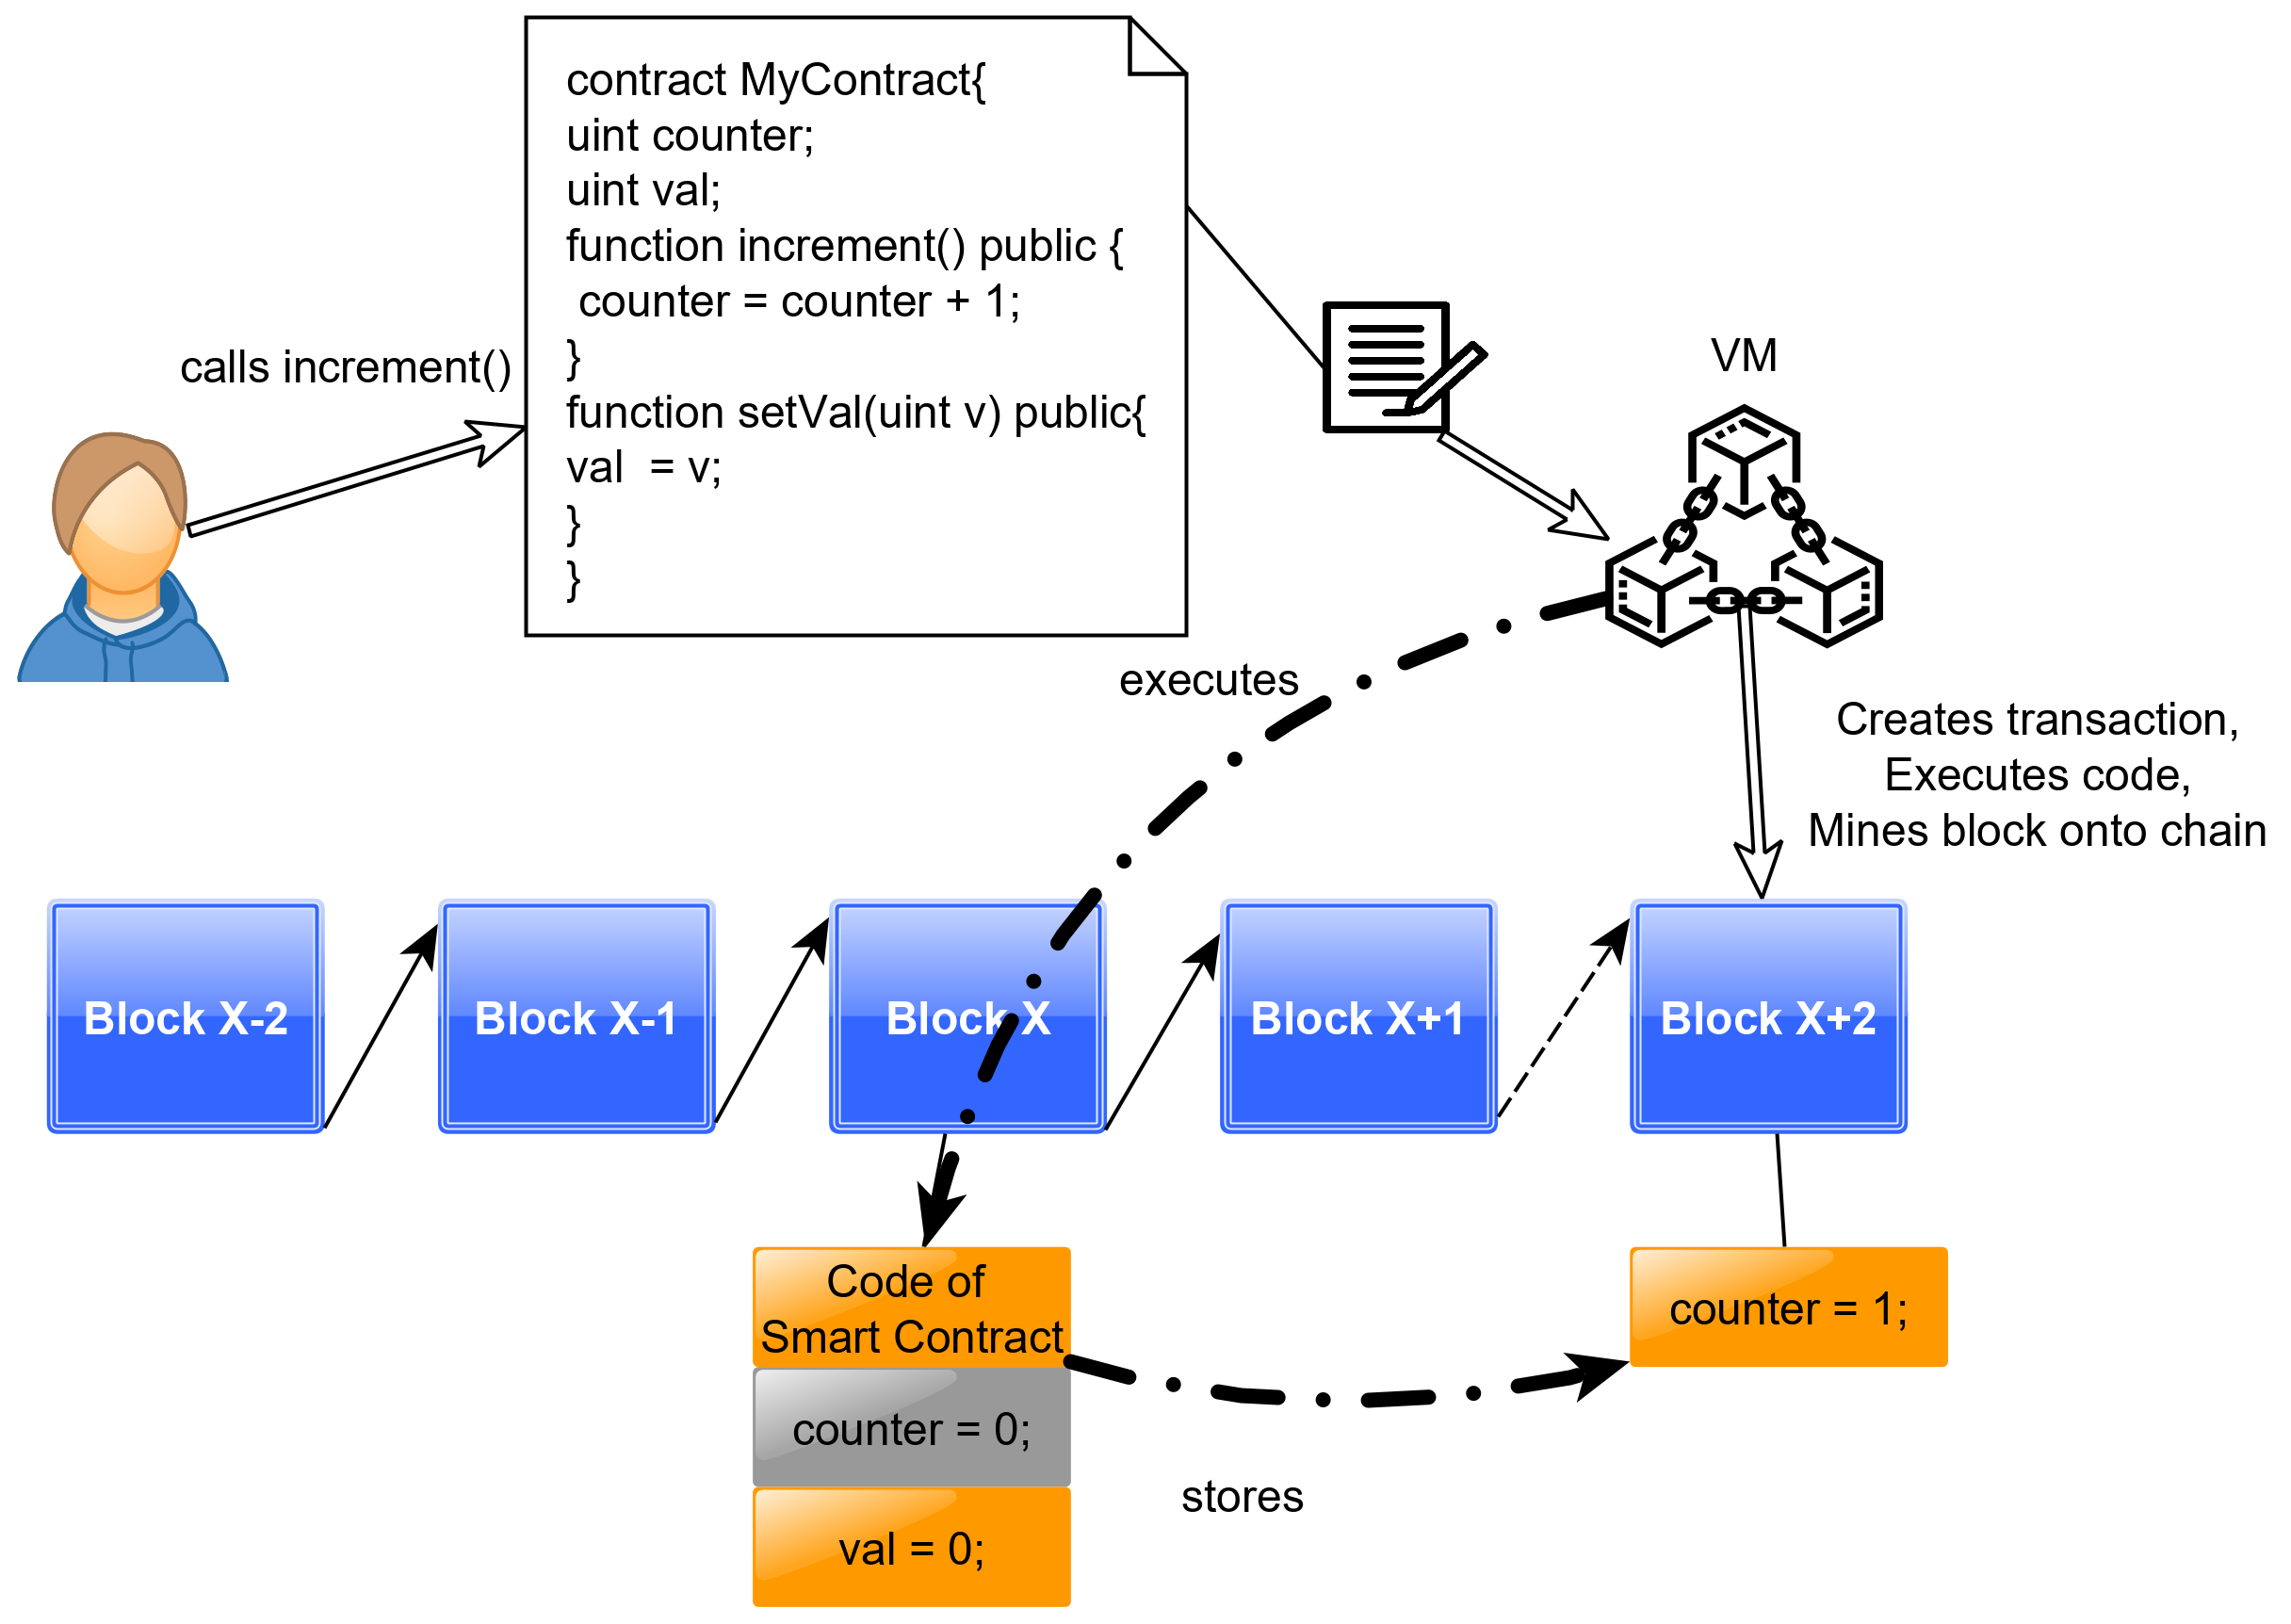
\includegraphics[width=0.9\textwidth]{figures/deploy_1.png}
    \caption{User calls a function of the smart contract, VM executes code, creates transaction, mines block onto the chain}
    \label{fig:deploy_1}
\end{figure}
\begin{figure}[H]
    \centering
    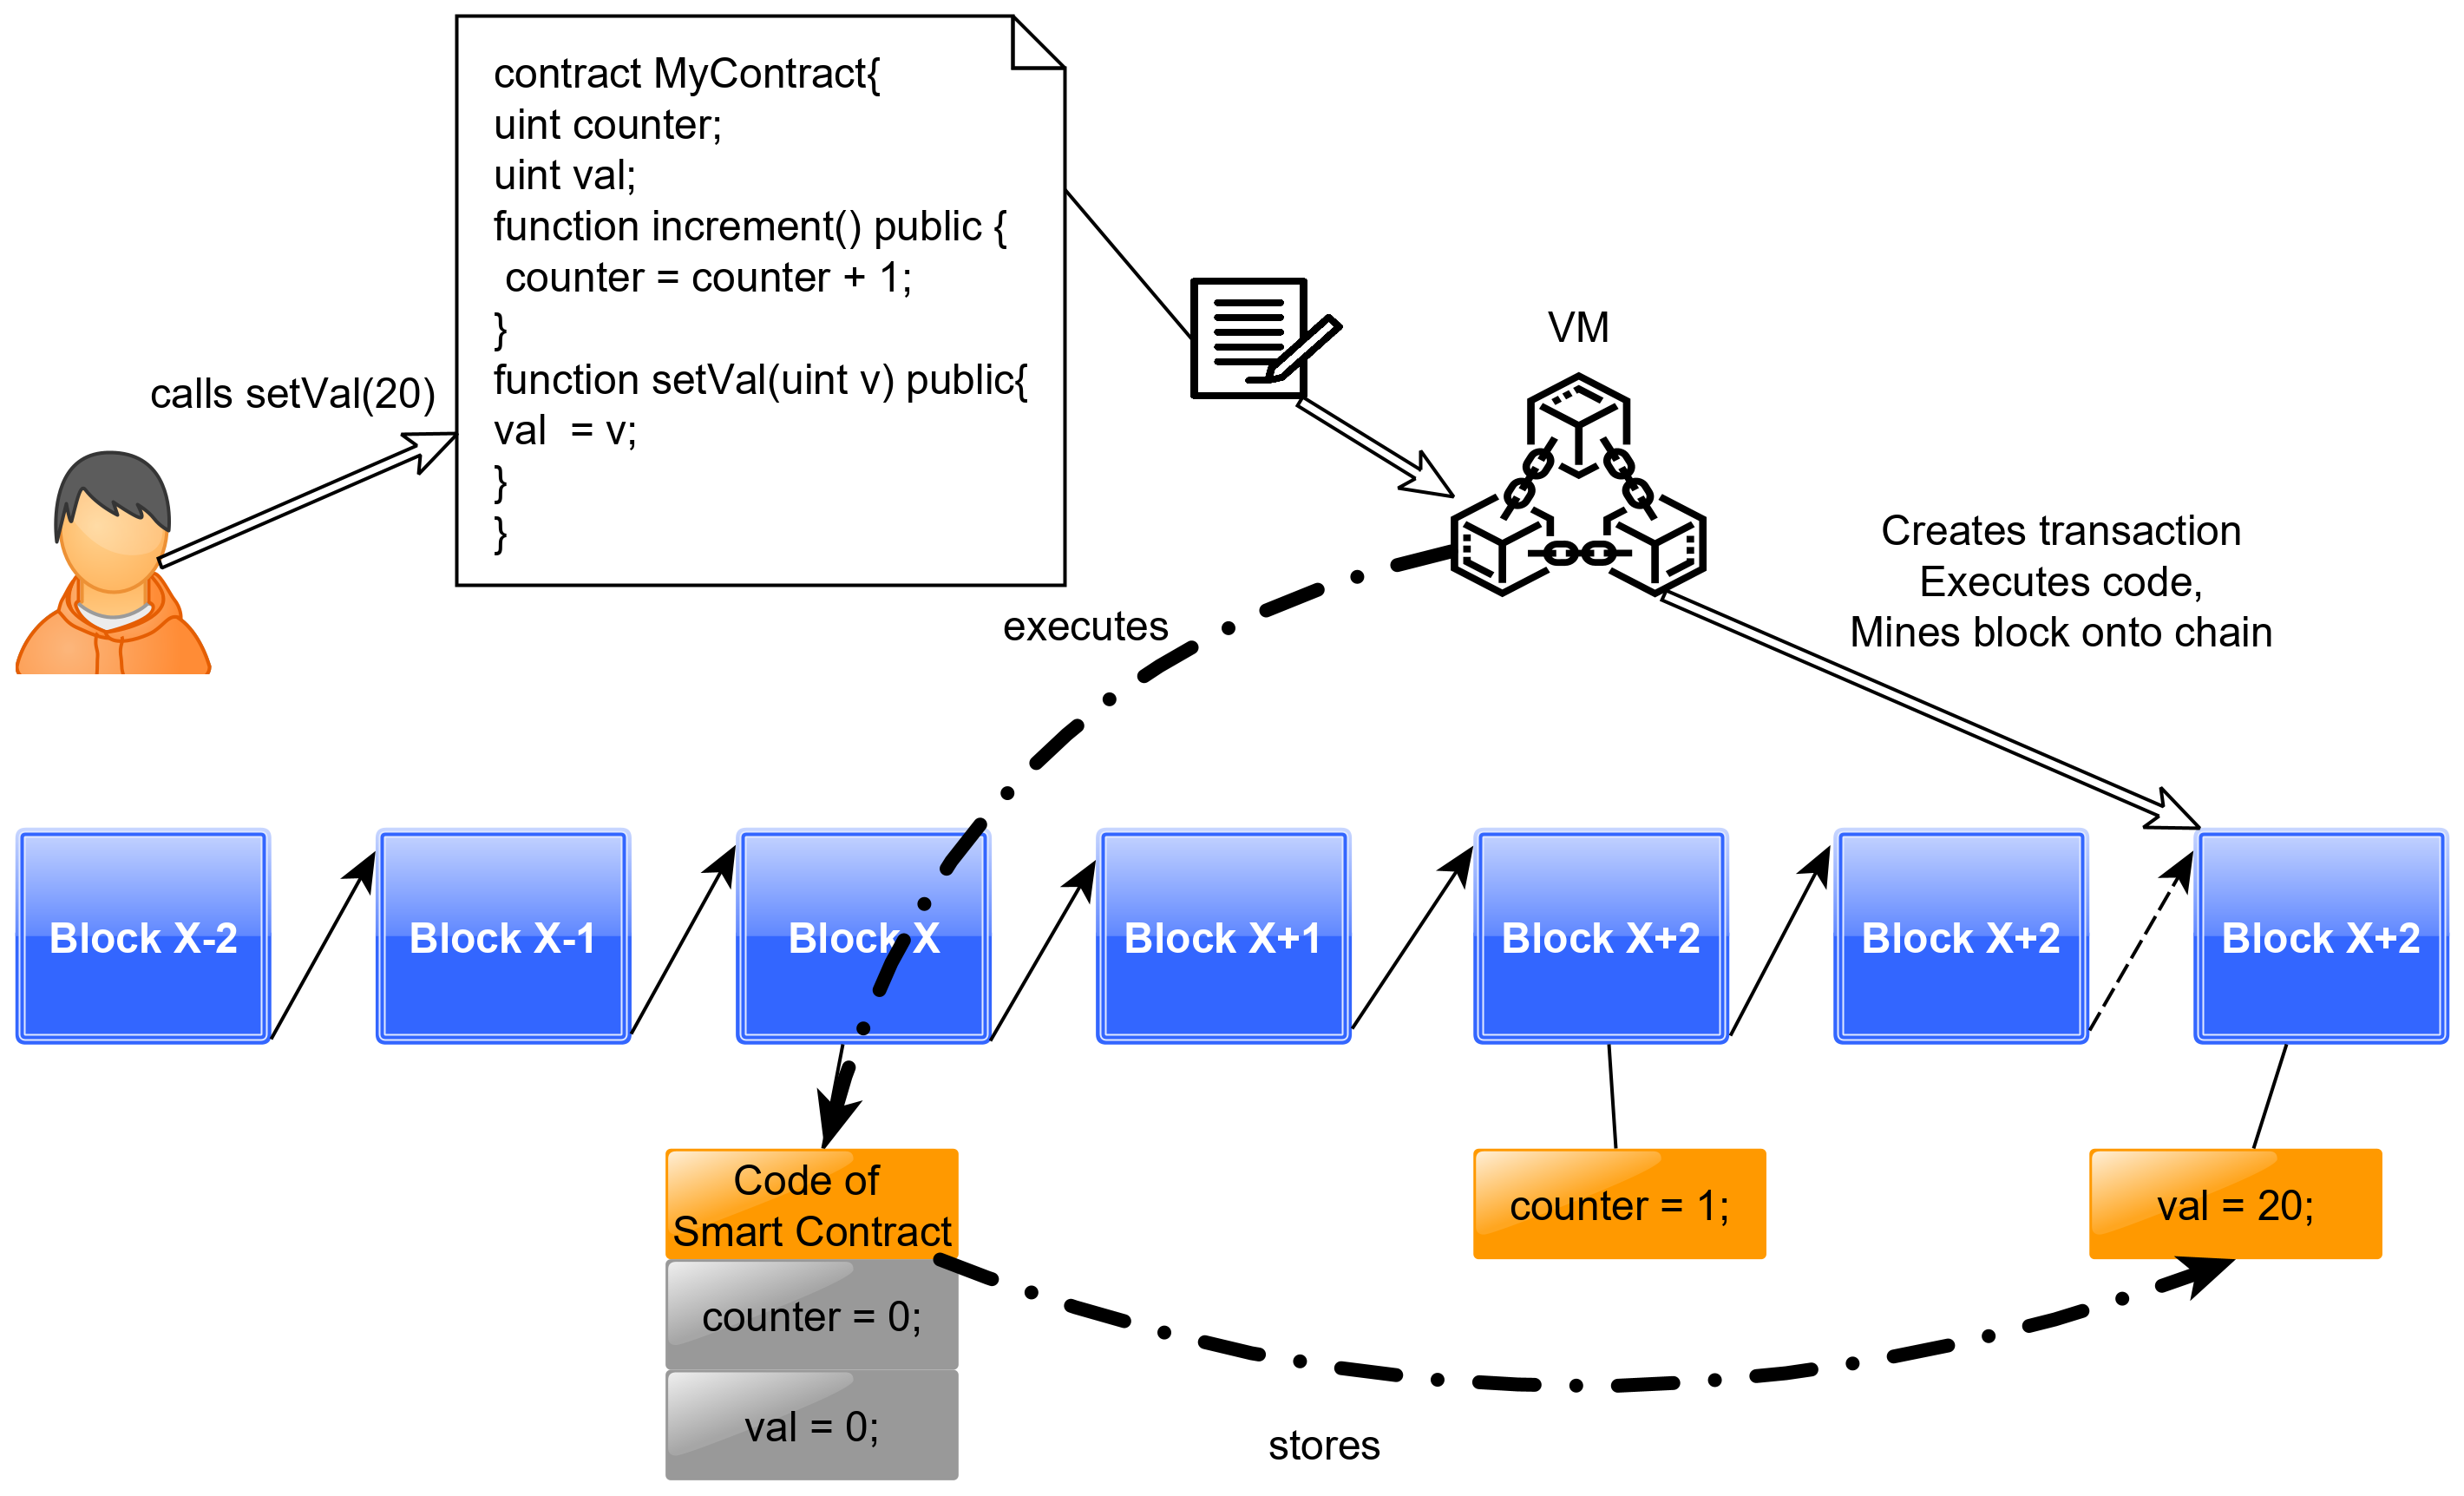
\includegraphics[width=0.9\textwidth]{figures/deploy_2.png}
    \caption{Another user calls a different function, at every time point, orange data members indicate a valid state of the contract object}
    \label{fig:deploy_1}
\end{figure}

\subsection{Solidity basics}

Solidity is an object-oriented, high-level language for implementing smart contracts. Smart contracts are programs which govern the behaviour of accounts within the Ethereum state. Solidity was influenced by C++, Python and JavaScript and is designed to target the Ethereum Virtual Machine (EVM).
Solidity is statically typed, supports inheritance, libraries and complex user-defined types among other features. With Solidity you can create contracts for uses such as voting, crowdfunding, blind auctions, and multi-signature wallets.\cite{solidity_manual}

\textbf{TODO: clean this up, add more references}


Contracts in Solidity are similar to classes in object-oriented languages. They contain persistent data in state variables and functions that can modify these variables. Calling a function on a different contract (instance) will perform an EVM function call and thus switch the context such that state variables are inaccessible. A contract and its functions need to be called for anything to happen. There is no “cron” concept in Ethereum to call a function at a particular event automatically.

Contracts can be created “from outside” via Ethereum transactions or from within Solidity contracts.

IDEs, such as Remix, make the creation process seamless using UI elements.

Creating contracts programmatically on Ethereum is best done via using the JavaScript API web3.js. It has a function called web3.eth.Contract to facilitate contract creation.

When a contract is created, its constructor (a function declared with the constructor keyword) is executed once.
A constructor is optional. Only one constructor is allowed, which means overloading is not supported.

After the constructor has executed, the final code of the contract is deployed to the blockchain. This code includes all public and external functions and all functions that are reachable from there through function calls. The deployed code does not include the constructor code or internal functions only called from the constructor.

Internally, constructor arguments are passed ABI encoded after the code of the contract itself, but you do not have to care about this if you use web3.js\cite{web3_api}.

Solidity is a statically typed language, which means that the type of each variable (state and local) needs to be specified. Solidity provides several elementary types which can be combined to form complex types.

The concept of “undefined” or “null” values does not exist in Solidity, but newly declared variables always have a default value dependent on its type. To handle any unexpected values, you should use the revert function to revert the whole transaction, or return a tuple with a second bool value denoting success.

Value Types
Fixed Point Numbers
Address address: Holds a 20 byte value (size of an Ethereum address).
address payable: Same as address, but with the additional members transfer and send
Contract Types
Fixed-size byte arrays
Function Types

Function types are the types of functions. Variables of function type can be assigned from functions and function parameters of function type can be used to pass functions to and return functions from function calls. Function types come in two flavours - internal and external functions:

Internal functions can only be called inside the current contract (more specifically, inside the current code unit, which also includes internal library functions and inherited functions) because they cannot be executed outside of the context of the current contract. Calling an internal function is realized by jumping to its entry label, just like when calling a function of the current contract internally.

External functions consist of an address and a function signature and they can be passed via and returned from external function calls.

Function types are notated as follows:

function (<parameter types>) {internal|external} [pure|view|payable] [returns (<return types>)]

Reference Types

Values of reference type can be modified through multiple different names. Contrast this with value types where you get an independent copy whenever a variable of value type is used. Because of that, reference types have to be handled more carefully than value types. Currently, reference types comprise structs, arrays and mappings. If you use a reference type, you always have to explicitly provide the data area where the type is stored: memory (whose lifetime is limited to a function call), storage (the location where the state variables are stored) or calldata (special data location that contains the function arguments, only available for external function call parameters).

An assignment or type conversion that changes the data location will always incur an automatic copy operation, while assignments inside the same data location only copy in some cases for storage types.
Data location

Every reference type, i.e. arrays and structs, has an additional annotation, the “data location”, about where it is stored. There are three data locations: memory, storage and calldata. Calldata is only valid for parameters of external contract functions and is required for this type of parameter. Calldata is a non-modifiable, non-persistent area where function arguments are stored, and behaves mostly like memory.

Data location and assignment behaviour

Data locations are not only relevant for persistency of data, but also for the semantics of assignments:

    Assignments between storage and memory (or from calldata) always create an independent copy.
    Assignments from memory to memory only create references. This means that changes to one memory variable are also visible in all other memory variables that refer to the same data.
    Assignments from storage to a local storage variable also only assign a reference.
    All other assignments to storage always copy. Examples for this case are assignments to state variables or to members of local variables of storage struct type, even if the local variable itself is just a reference.

Structs
Solidity provides a way to define new types in the form of structs, which is shown in the following example:
Mapping Types

You declare mapping types with the syntax mapping(KeyType => ValueType). The KeyType can be any elementary type. This means it can be any of the built-in value types plus bytes and string. User-defined or complex types like contract types, enums, mappings, structs and any array type apart from bytes and string are not allowed. ValueType can be any type, including mappings.

You can think of mappings as hash tables, which are virtually initialised such that every possible key exists and is mapped to a value whose byte-representation is all zeros, a type’s default value. The similarity ends there, the key data is not stored in a mapping, only its keccak256 hash is used to look up the value.

Because of this, mappings do not have a length or a concept of a key or value being set, and therefore cannot be erased without extra information regarding the assigned keys (see Clearing Mappings).

Constructor, method, view, nonpayable, payable, data types, storage locations, best practices, references 

Development (mention remix IDE)

\section{Introduction to the demo environment}

The following tools are \textbf{required} in order to effectively participate in the tutorial
\begin{itemize}
    \item Web browser supporting ECMAScript 2015
    \item SSH client (e.g. \emph{putty} on windows, \emph{openssh} on linux
    \item Arbitrary text editor for Solidity smart contract editing
\end{itemize}{}

The \href{https://blockchain.cnsm2019-tutorial.com/}{demo environment} - as illustrated by Figure \ref{fig:demo-env} - consists of a Web UI and back-end for managing the training sessions and allowing that the participants can easily interact with each other's deployed contracts.The back-end interacts with the Etherum based blockchain network using web3 API. The blockchain network consists only one node for now, but that doesn't greatly affects how the endpoints would interact with the blockchain network as long as connection is available to a node.

\begin{figure}[H]
    \centering
    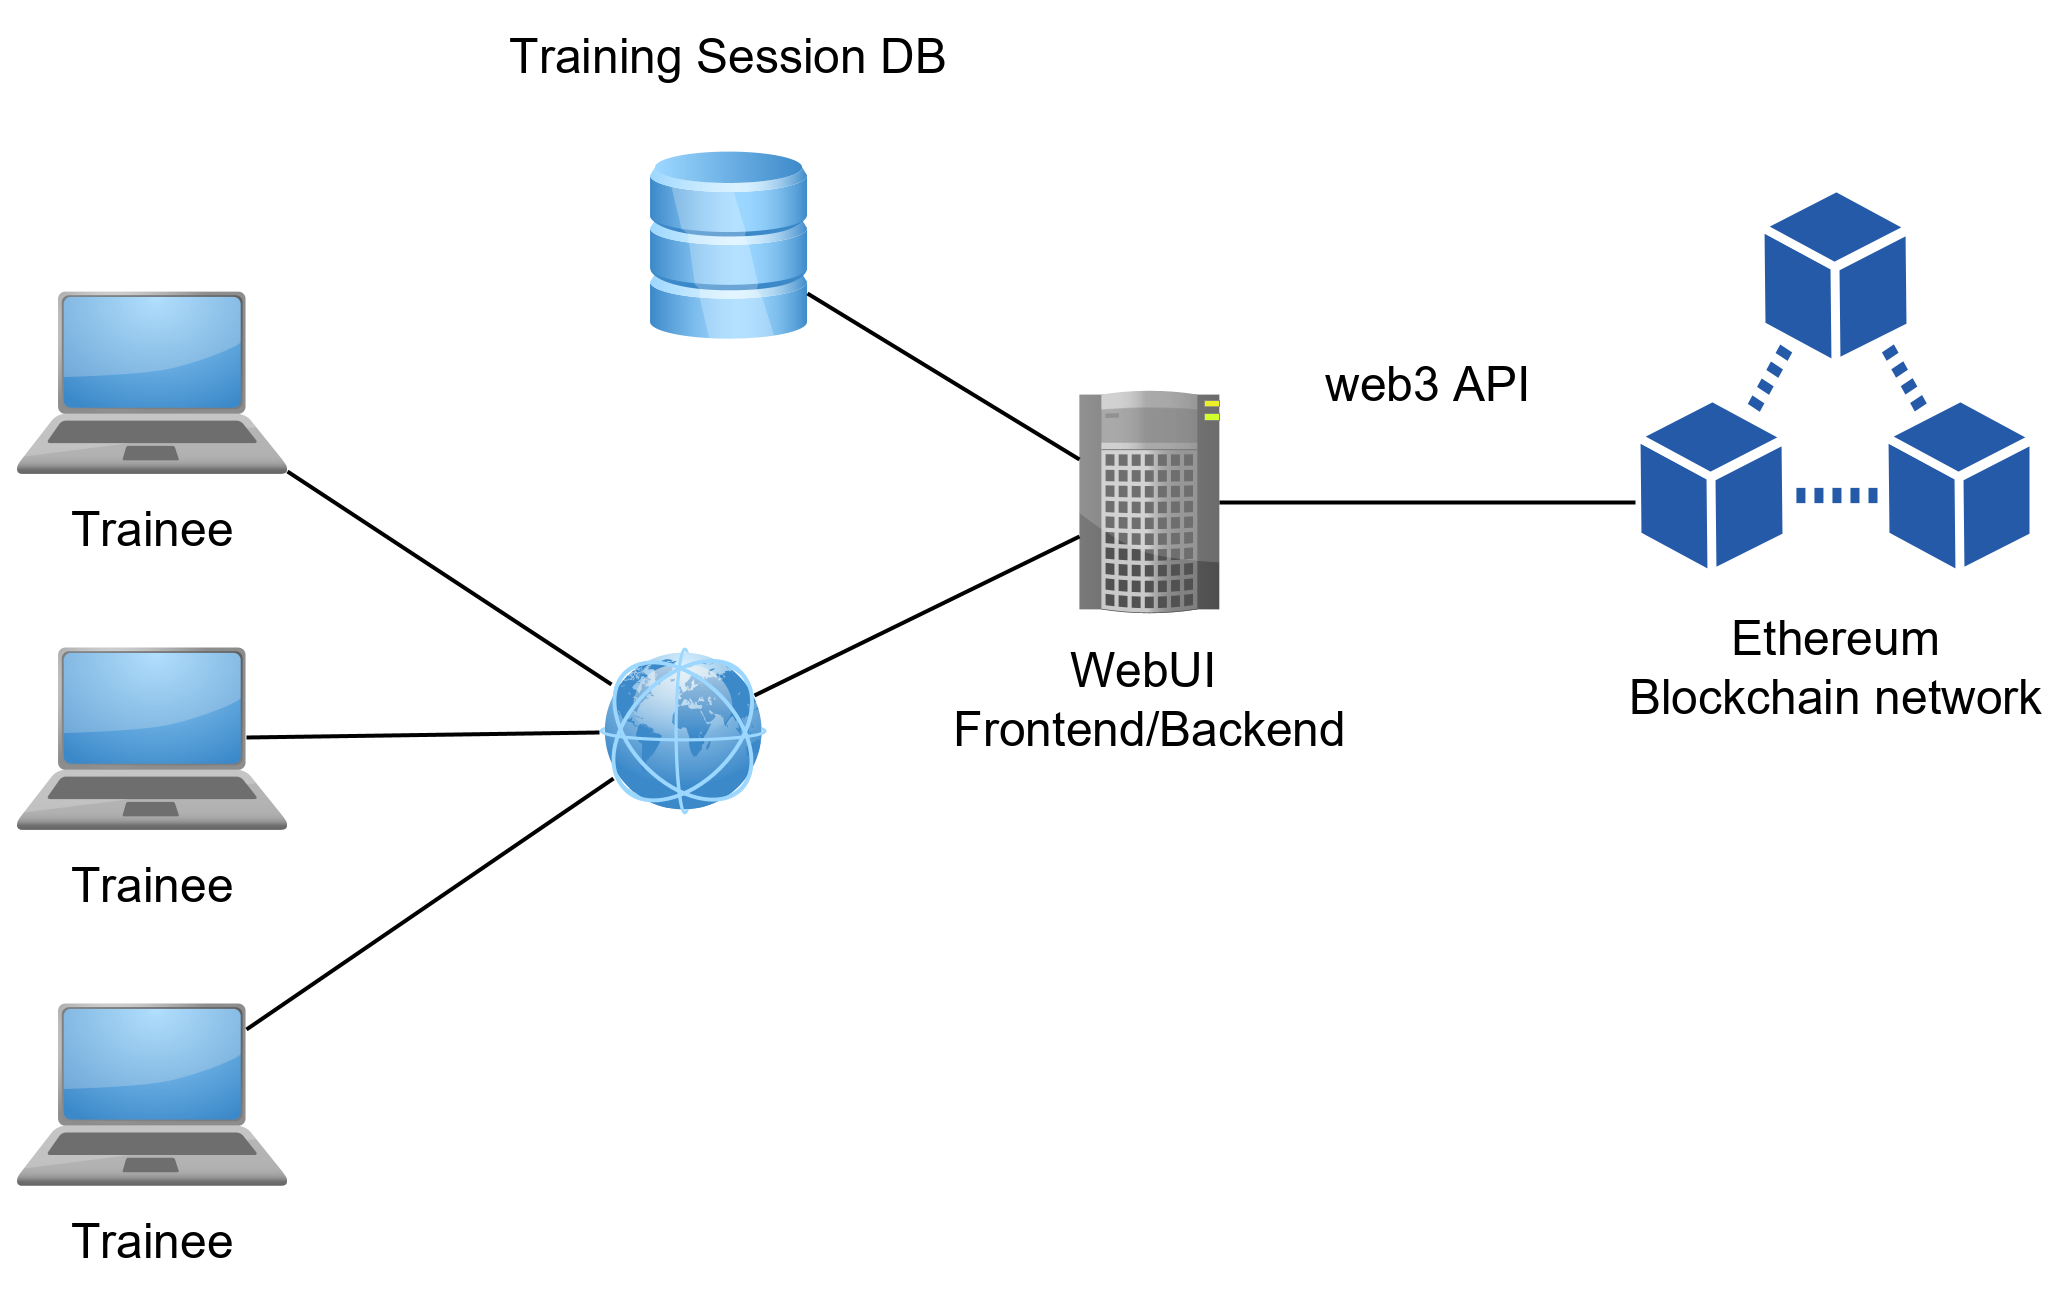
\includegraphics[width=0.9\textwidth]{figures/env.png}
    \caption{The tutorial environment}
    \label{fig:demo-env}
\end{figure}

Registration is available, but at the beginning of the hands-on part of the tutorial the participants will receive usernames and passwords to use as that accounts will be pre-filled so that contract deployment can be performed right away.

For using the \texttt{geth} console the participants are expected to be able to login to \url{ssh://tutorial@blockchain.cnsm2019-tutorial.com:2222} i.e. SSH using port \textbf{2222} and using username \texttt{tutorial} to host \url{blockchain.cnsm2019-tutorial.com}. The password to be used will be provided during the tutorial session.

\section{Tutorial exercises}

\subsection{Verify logins}

\begin{enumerate}[label=\textbf{Task \arabic*}:, series=l_tasks]
\item login both to the WebUI and to the backend host using ssh.
\end{enumerate}

After logging in to the web page, you should see your ethereum account's address in the top left portion of the screen(see Figure \ref{fig:login-user-acc}). After this step verify that you are able to log in using SSH to the back-end.

\begin{figure}[H]
    \centering
    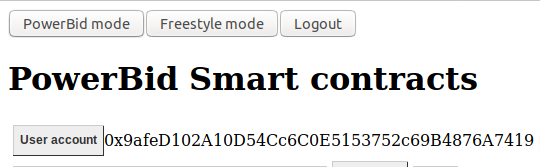
\includegraphics[width=0.6\textwidth]{figures/login-useracc.png}
    \caption{Displayed user account}
    \label{fig:login-user-acc}
\end{figure}

\begin{enumerate}[label=\textbf{Task \arabic*}:,l_tasks]
\item Check your balance using the \texttt{geth} node in console mode using commands found in listings \ref{lst:attach} and \ref{lst:balance}
\end{enumerate}

\begin{lstlisting}[language=bash,caption={attach to geth node},label={lst:attach}]
sudo ./admin/geth_attach 
\end{lstlisting}

\begin{lstlisting}[language=javascript,caption={Function for checking balance},label={lst:balance}]
account="0x31773dE44FD9683F56C7aE7ea0e8bf3Ba7b9F717" //replace with your account
eth.getBalance(account)
\end{lstlisting}

You should see a number greater than 0. The \verb!geth! console is a javascript REPL and essentially the commands that can be used are the ones the web3 API exposes. For further reference of functions please study the corresponding \href{https://web3js.readthedocs.io/en/v1.2.1/web3.html}{web3 API documentation}.


After successful execution something similar should be seen:
\begin{verbatim}
tutorial@87cd2f75a465:~$ sudo ./admin/geth_attach 
[sudo] password for tutorial: 
Welcome to the Geth JavaScript console!

instance: Geth/v1.9.1-stable-b7b2f60f/linux-amd64/go1.12.7
coinbase: 0xf5573ac8504e8280c43806c156ff52984bc35c16
at block: 1133 (Sun, 13 Oct 2019 10:08:50 UTC)
 datadir: /iot_sc_tutorial/datadir
 modules: admin:1.0 debug:1.0 eth:1.0 ethash:1.0 miner:1.0 net:1.0 personal:1.0 rpc:1.0 txpool:1.0 web3:1.0

> eth.getBalance("0x9afeD102A10D54Cc6C0E5153752c69B4876A7419")
1e+22
> 
\end{verbatim}

As one can notice this \verb!eth.getBalance! function returns the balance in \emph{Wei} dimension. There's a utility function called \verb!web.toWei! in the web3 module which can be used to transform between units e.g. to get the balance in \emph{ether} the following can be executed:
\begin{verbatim}
> eth.getBalance(account)/web3.toWei(1,"ether")
10000
> 
\end{verbatim}


\subsection{Transactions using the console}

As a next step we will initiate transactions using the \verb!geth! console.

\begin{enumerate}[label=\textbf{Task \arabic*}:,l_tasks]
\item Select one of your peers as recipient and transfer 1 ether to them using the console. Check your balance before and after the transaction. The corresponding function to use is \ref{lst:balance} and \ref{lst:transfer}
\end{enumerate}

\begin{lstlisting}[language=javascript,caption={Functions to be used for signing and sending a transaction},label={lst:transfer}]
myself="0x9afeD102A10D54Cc6C0E5153752c69B4876A7419" // replace with your account
recipient="0x3FecF304285303Fba1C34124889Ea1256e9BB0de" // replace with the target account
password="user1" // replace with your password

signedTransaction = personal.signTransaction({
    from: myself,
    to: recipient,
    value: web3.toWei(1,"ether"),
    gas: 200000, 
    gasPrice:eth.gasPrice,
    nonce: eth.getTransactionCount(myself)
    },password )


transactionId = eth.sendRawTransaction(signedTransaction.raw)

eth.getTransaction(transactionId)
\end{lstlisting}

It could be that initial result of the transaction data might not contain the block hash and block number as it is in pending. In such case repeat the \verb!eth.getTransaction(transactionId)! command until those fields are populated

\begin{enumerate}[label=\textbf{Task \arabic*}:,l_tasks]
\item Analyze the block that contains your previous transaction, and check which other transactions might reside in the same block as yours using the commands in listing \ref{lst:block}
\end{enumerate}

\begin{lstlisting}[language=javascript,caption={Functions for analyzing a block},label={lst:block}]
eth.getBlock(eth.getTransaction(transactionId).blockNumber)

eth.getBlock(eth.getTransaction(transactionId).blockNumber).transactions.map(function(tx){return eth.getTransaction(tx);})
\end{lstlisting}

\subsection{PowerBid game}

\subsubsection{Description of the contract}
As part of familiarizing ourselves with the concepts of smart contracts and their potential use cases in IoT environments we are going to use a game. The game consists of a pre-implemented and simple smart contract that is modelling an electrical power auction. The game has 2 roles: supplier and consumer. The contract is created by the consumer where he specifies the required energy and the approximate time window where he intends to consume the required power. The creator - i.e. the consumer - of the contract also specifies a maximum price to pay for this amount of energy at that time window the he also has to pay upfront as a collateral to the deal. The suppliers essentially then monitor these contracts whether they can satisfy them while maximizing their profit then bid accordingly. This model is a sell auction i.e. a smaller price is considered more aggressive. 

The contract has been described in Solidity language and it's latest source that is used during this tutorial can be studied here: \url{https://raw.githubusercontent.com/fecjanky/iot_sc_tutorial/master/src/powerbid.sol}.

The contract has the following main phases:
\begin{enumerate}
    \item Auction Phase, where the suppliers participate in the sell auction
    \item Consumption Phase, where the consumer consumes the power paid and requested
    \item Withdraw Phase, where the consumer can withdraw his gain (that is the difference between the max. price and the best price) and the supplier can withdraw the funds from the contract
\end{enumerate}


\begin{figure}[H]
    \centering
    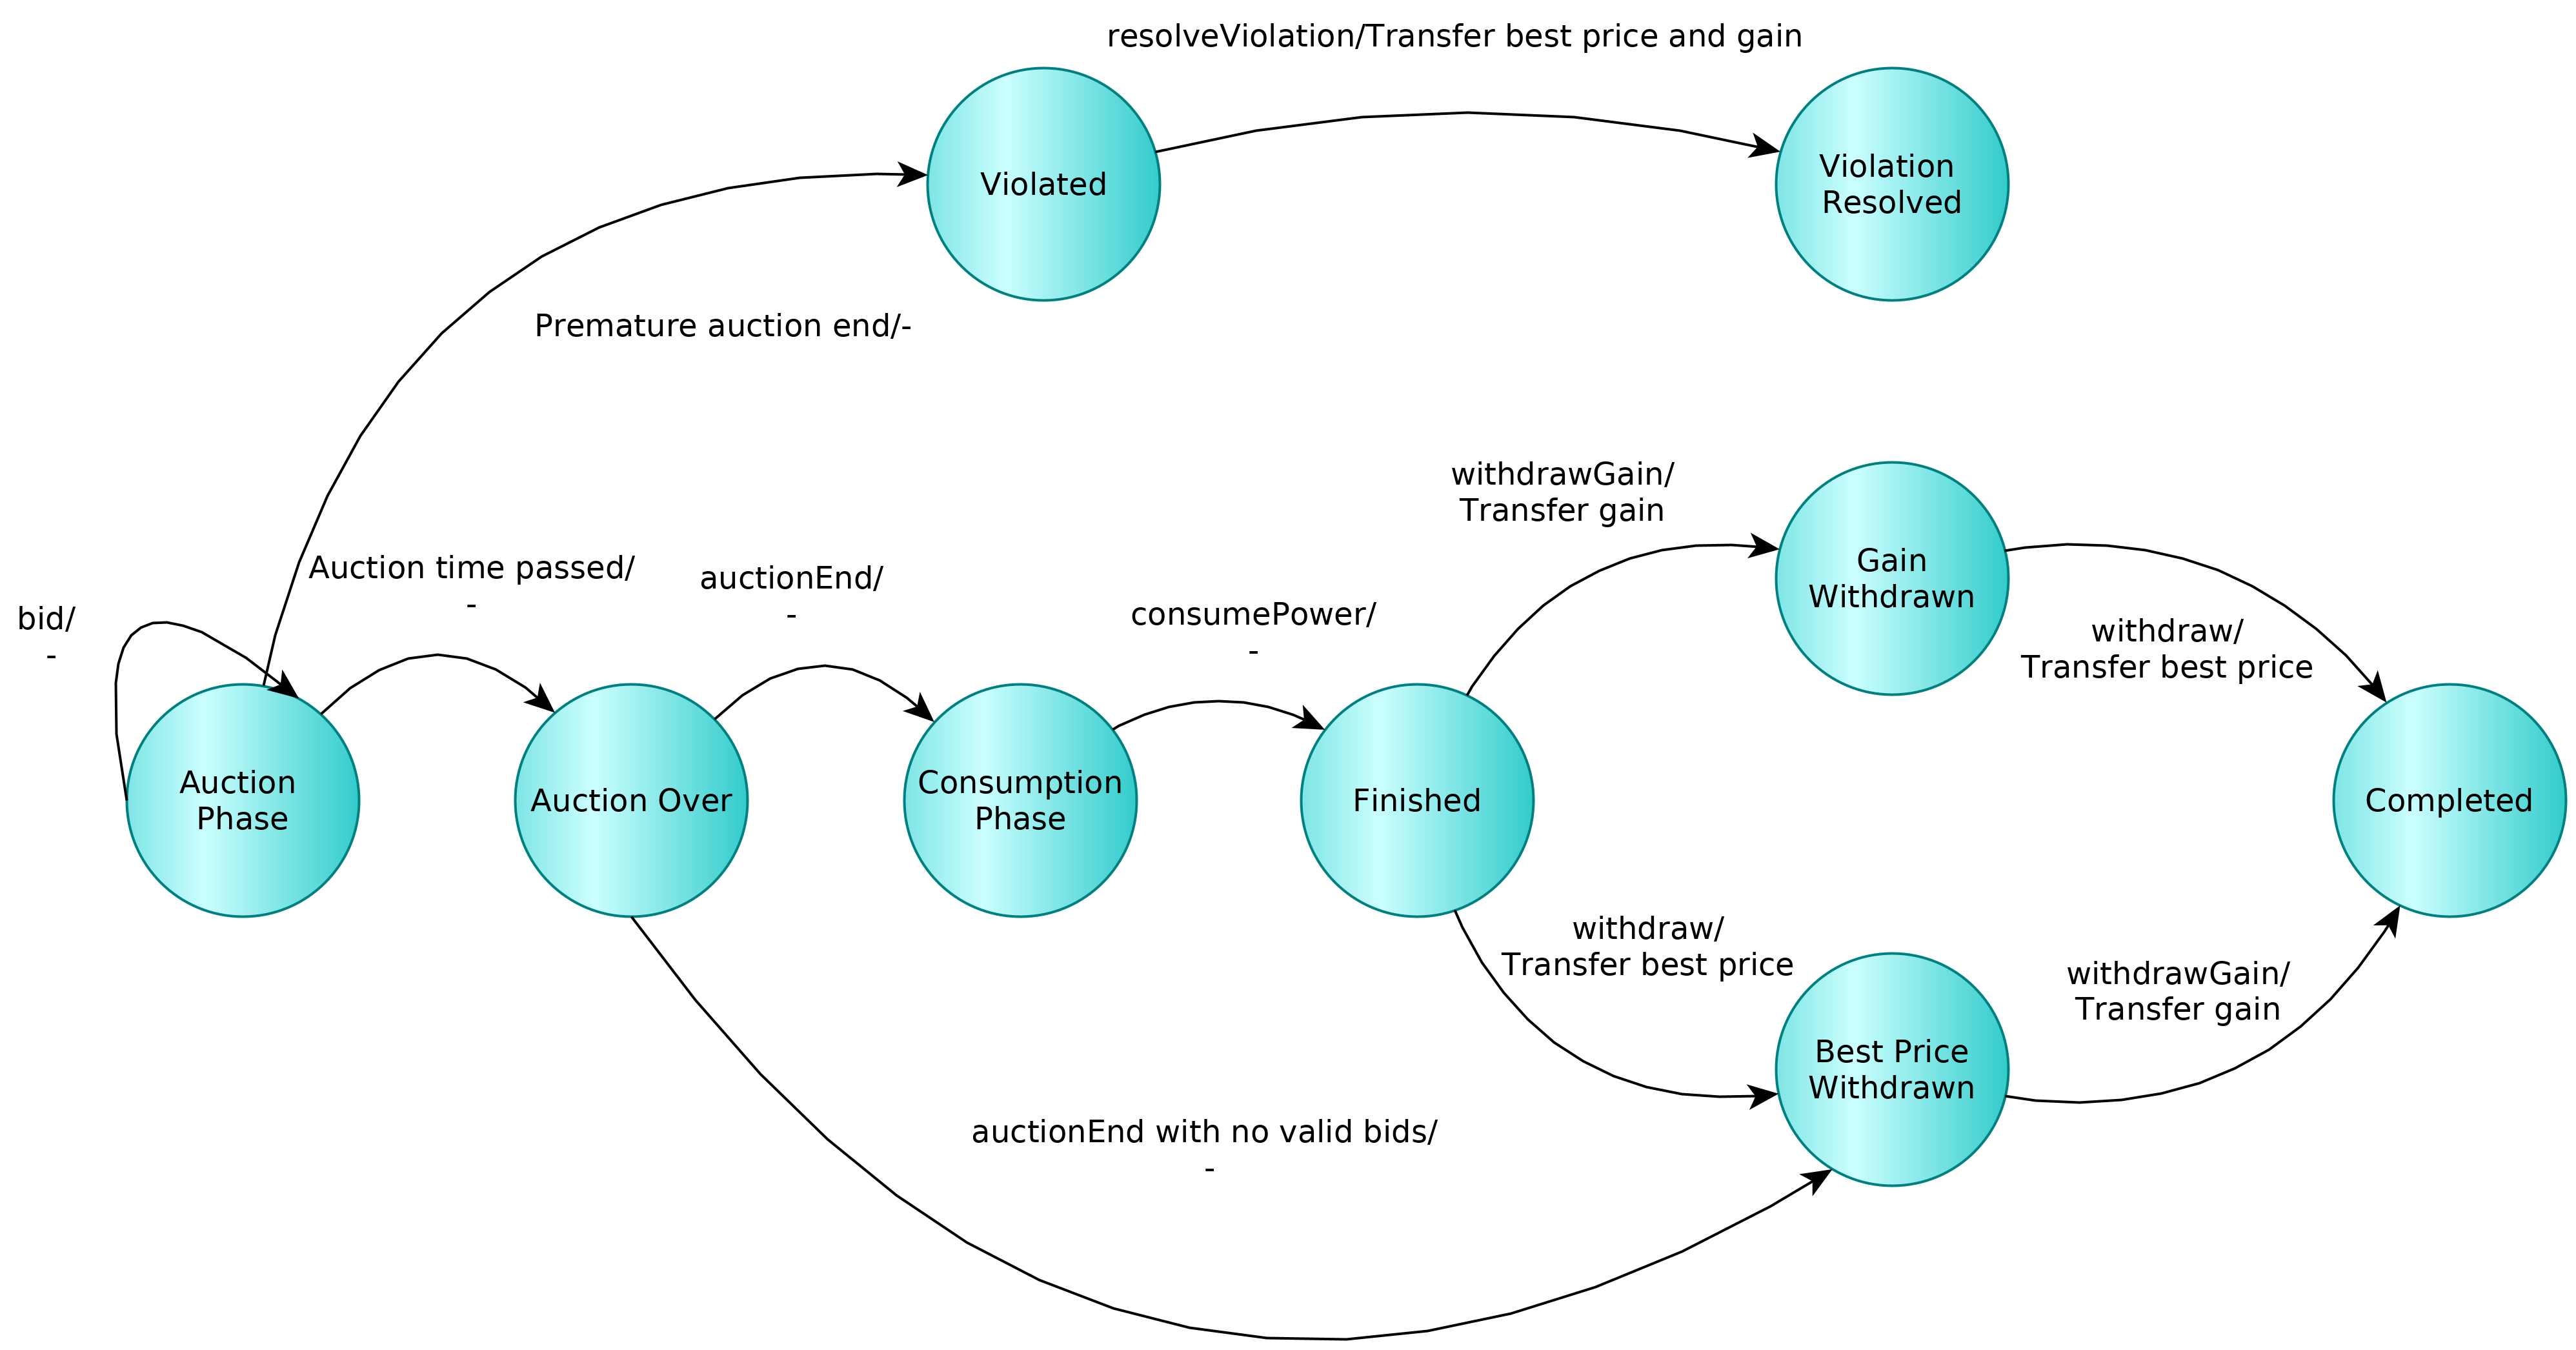
\includegraphics[width=0.9\textwidth]{figures/state_diagram.png}
    \caption{The state diagram of the PowerBid smart contract}
    \label{fig:State-diagram-powerbid}
\end{figure}

\subsubsection{Deployment, bidding and evaluation}

The deployment of contract is done by supplying the required constructor parameters in the row where the \emph{Deploy} button is present. The transaction options are sourced from the corresponding \emph{TX Options} inputs and mapped to the transaction parameters as supplied in one of the previous tasks (see listing \ref{lst:transfer}. The deployment is initiated by clicking the \emph{Deploy} button. After successful deployment (see Figure \ref{fig:deploy-powerbid}) the new contract will appear under the deployed contracts list on the left hand side and will be selected as the active contract. In this case the transaction receipt will be logged in the bottom grey log area while in case of error the error message has to be inspected to see what went wrong with the deployment.


\begin{figure}[H]
    \centering
    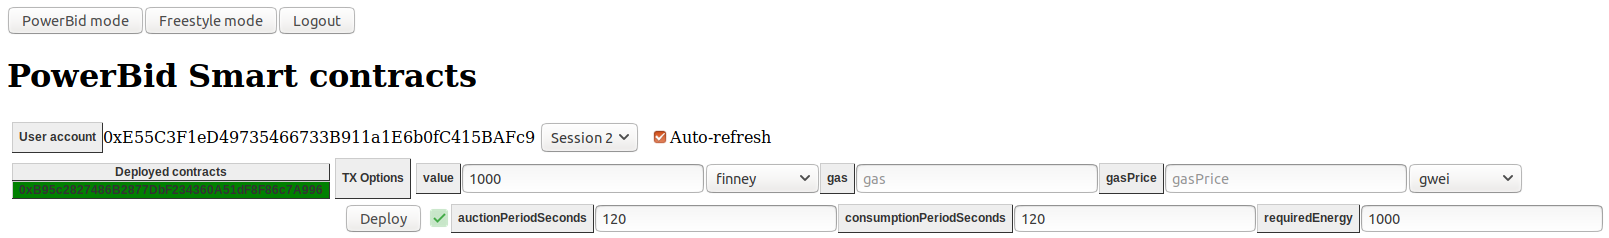
\includegraphics[width=0.9\textwidth]{figures/ui-deploy.png}
    \caption{Deployment of a Powerbid contract}
    \label{fig:deploy-powerbid}
\end{figure}

The \emph{TX Options} are not mandatory in case of an arbitrary smart contract but as one inspects the constructor code (see listing \ref{lst:powerbid-ctor}) it can be seen that  the message value must be greater than 0 \emph{Wei} i.e. the creator of this smart contract must transfer some money upfront that is in line how the auction is modelled. The \emph{gas} and \emph{gasPrice} options are not mandatory, and in that case those are estimated automatically using the web3 API. 

\begin{lstlisting}[language=javascript,caption={Excerpt from the constructor of the Powerbid smart contract},label={lst:powerbid-ctor}]
    constructor(
        uint auctionPeriodSeconds,
        uint consumptionPeriodSeconds,
        uint requiredEnergy
    ) public payable {
        require(requiredEnergy > 0, "required energy must be greater than 0 wh");
        require(msg.value > 0 ,"max price must be greater than 0");
        require(auctionPeriodSeconds > 0, "auction period must be greater than 0");
        require(consumptionPeriodSeconds > 0, "consumption period must be greater than 0");
        consumer = msg.sender;
        ...
    }
\end{lstlisting}

As described in section \ref{sec:EthSmartContracConcepts} the \emph{gas} determines the amount of operations that can be performed by the virtual machine while executing a give smart contract API call and the \emph{gasPrice} will be the reward of the individual who successfully places the transaction in a block onto the canonical chain. For these exercises the \emph{gas} field can be left empty, however the \emph{gasPrice} should be specified as if it is missing it will be estimated based on the last few blocks median gas price and depending on the exchange values it can happen easily that the transaction costs more than the gained value resulting in a net balance decrease.

It's also worth mentioning that in case of a \verb!require! expression failure in the code when the transaction would be normally reverted the estimation will always fail with the same error message \emph{'gas required exceeds allowance (8000000) or always failing transaction'}, while if no estimation is needed - i.e. all options are specified, then the EVM will try to create the transaction, but it will result in a reversion due to the failed assertion with error \emph{'Transaction has been reverted by the EVM'} (see Figures \ref{fig:deploy-error-est} and \ref{fig:deploy-error-noest}). In both cases the contract's source code has to be studied for further troubleshooting. As of the time of this writing the \verb!require! expression's string parameter is not propagated to the user, but that can change in the future editions of the tool-chain as a consequence it is good practice to give meaningful diagnostics there.

\begin{figure}[H]
    \centering
    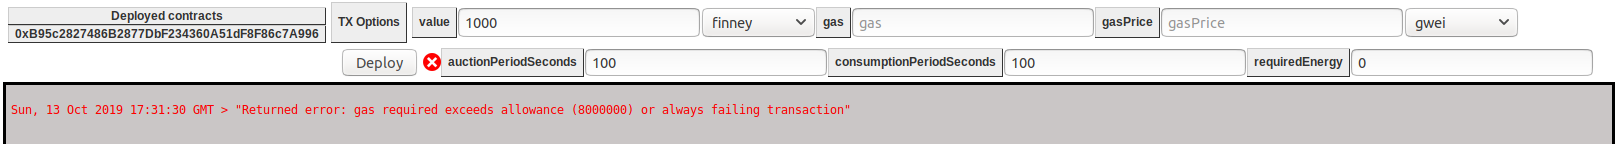
\includegraphics[width=0.9\textwidth]{figures/error-withestimation.png}
    \caption{Invalid parameters with estimation}
    \label{fig:deploy-error-noest}
\end{figure}

\begin{figure}[H]
    \centering
    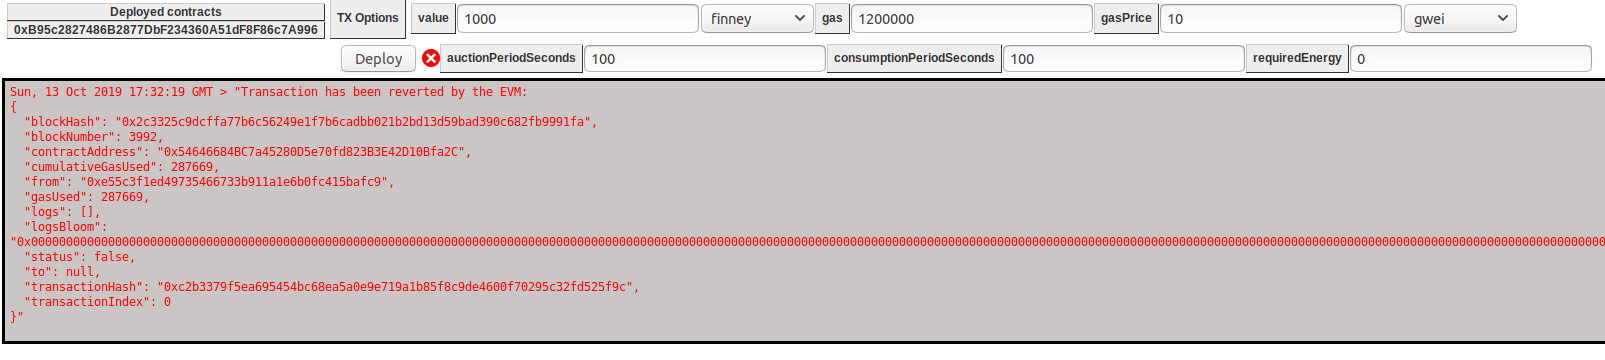
\includegraphics[width=0.9\textwidth]{figures/error-noestimation.png}
    \caption{Invalid parameters without estimation}
    \label{fig:deploy-error-est}
\end{figure}


After successful deployment the contract will show up on the left hand side listing. By clicking on a deployed contract it's controls will become visible. The auction and consumption time left fields are updated automatically, but the other fields have to be queried manually by either calling the corresponding API function (exposed as the adjacent button) or by clicking on the phase getter, that will call all non-mutable API functions. The functions that mutate the contract are marked red. The suppliers can use the \emph{bid} function to place their bids.

After the auction period has ended the consumption phase begins. The consumer can end the auction prematurely but in that case a different state transition sequence begins (see Figure \ref{fig:State-diagram-powerbid}.

After the consumption period has passed or the consumer explicitly marked the contract as consumed by clicking on the \emph{consumePower} button the contract is open for withdrawals. The amounts can be withdrawn in any order driving the contract into the \emph{Completed} state which is a terminal state.


\begin{enumerate}[label=\textbf{Task \arabic*}:,l_tasks]
\item After deploying a contract check its balance to clearly see that the money is upfront allocated. Observe the balance changes after every phase. \ref{lst:block}
\end{enumerate}

\subsubsection{Game-play summary}

The high-level game-play for the two different roles can be summarized as:
\begin{itemize}
    \item Consumer role:
    \begin{enumerate}
        \item Deploy contract after specifying the constructor parameters
        \item Monitor the sell auction until the auction is ongoing.
        \item Consume the power (virtually, calling the \emph{'consumePower'} API by pressing the corresponding button)
        \item withdraw gains (Max. price - best price)
        \item evaluate relative gain
    \end{enumerate}
    \item Producer/Supplier role:
    \begin{enumerate}
        \item Bid on the deployed Smart contracts
        \item monitor bid state based on the visual feedback and/or polling the contracts
        \item place further bids as desired
        \item wait for consumer to consume the power
        \item withdraw the price amount from the contracts that has been win by the user
        \item evaluate relative gain
    \end{enumerate}
\end{itemize}

TODO: describe interaction, game params and evaluation
TODO: specify tasks: deploy, bid, analyze transactions, etc.

\subsection{Implement a number guessing game}

\subsubsection{Specification}

The game participants are guessing numbers. The winner is who choose the smallest number. If a number has been chosen by more than 1 person it is not considered as a valid guess. 1 person can only guess once. The creator offers a prize that (greater than 0 Wei) is to be won by the winner. If at the end of the game there are no valid guesses the creator is considered the winner. Only the winner must be able to withdraw the prize. At construction time the owner should be able to specify the total number of guesses that will limit the number of individuals who are able to play the game. The prize mustn't be possible to be withdrawn before the game ends. The results should only be possible to be queried through the programmatic API when the game is over.

\subsection{Template}

\section*{Acknowledgement}
This Tutorial has been initially compiled for the audience of the 15th International Conference on Network and Service Management -- technically co-sponsored by IFIP, IEEE Communication Society, IEEE Computer Society, and ACM.

In connection to this work, the authors have received funding  from  the  EU  ECSEL JU under the H2020 Framework Programme, JU grant nr.  737459  (Productive4.0  project,  www.productive40.eu).
Part of this work was supported by the Higher Education Excellence  Program  of  the  Ministry  of  Human  Capacities, Hungary, in the frame of Artificial Intelligence research area of Budapest University of Technology and Economics (BME FIKP-MI/SC). 

\bibliographystyle{ieeetr}
\bibliography{references}

\end{document}